\documentclass[a4paper, 12pt]{report}
\usepackage{cmap}
\usepackage{amssymb}
\usepackage{amsmath}
\usepackage{graphicx}
\usepackage{amsthm}
\usepackage{upgreek}
\usepackage{setspace}
\usepackage{color}
\usepackage{moreverb}
\usepackage[T2A]{fontenc}
\usepackage[utf8]{inputenc}
\usepackage[normalem]{ulem}
\usepackage{mathtext} % русские буквы в формулах
\usepackage[left=2cm,right=2cm, top=2cm,bottom=2cm,bindingoffset=0cm]{geometry}
\usepackage[english,russian]{babel}
\usepackage[unicode]{hyperref}
\newenvironment{Proof} % имя окружения
{\par\noindent{$\blacklozenge$}} % команды для \begin
{\hfill$\scriptstyle\boxtimes$}
\newcommand{\Rm}{\mathbb{R}}
\newcommand{\Cm}{\mathbb{C}}
\newcommand{\Z}{\mathbb{Z}}
\newcommand{\I}{\mathbb{I}}
\newcommand{\N}{\mathbb{N}}
\newcommand{\rank}{\operatorname{rank}}
\newcommand{\Ra}{\Rightarrow}
\newcommand{\ra}{\rightarrow}
\newcommand{\FI}{\Phi}
\newcommand{\Sp}{\text{Sp}}
\renewcommand{\leq}{\leqslant}
\renewcommand{\geq}{\geqslant}
\renewcommand{\alpha}{\upalpha}
\renewcommand{\beta}{\upbeta}
\renewcommand{\gamma}{\upgamma}
\renewcommand{\delta}{\updelta}
\renewcommand{\varphi}{\upvarphi}
\renewcommand{\phi}{\upvarphi}
\renewcommand{\tau}{\uptau}
\renewcommand{\lambda}{\uplambda}
\renewcommand{\psi}{\uppsi}
\renewcommand{\mu}{\upmu}
\renewcommand{\omega}{\upomega}
\renewcommand{\d}{\partial}
\renewcommand{\xi}{\upxi}
\renewcommand{\epsilon}{\upvarepsilon}
\newcommand{\intx}{\int\limits_{x_0}^x}
\newcommand\Norm[1]{\left\| #1 \right\|}
\newcommand{\sumk}{\sum\limits_{k=0}^\infty}
\newcommand{\sumi}{\sum\limits_{i=0}^\infty}
\newtheorem*{theorem}{Теорема}
\newtheorem*{cor}{Следствие}
\newtheorem*{lem}{Лемма}
\begin{document}
	% Оформление титульного листа
	\begin{titlepage}
		\begin{center}
			\textsc{МИНИСТЕРСТВО ОБРАЗОВАНИЯ РЕСПУБЛИКИ БЕЛАРУСЬ БЕЛОРУССКИЙ ГОСУДАРСТВЕННЫЙ УНИВЕРСИТЕТ
				\\[5mm]
				ФАКУЛЬТЕТ ПРИКЛАДНОЙ МАТЕМАТИКИ И ИНФОРМАТИКИ\\[2mm]
				Кафедра информационных систем управления
			}
			
			\vfill
			
			\textbf{Отчет по лабораторной работе №1\\
				Вариант 52
				\\[26mm]
			}
		\end{center}
		
		\hfill
		\begin{minipage}{.5\textwidth}
			\begin{flushright}
				Бовта Тимофея Анатольевича\\
				студента 3 курса\\
				специальности «прикладная математика»\\[5mm]
				
				Преподаватель:\\[2mm] 
				Д. Ю. Кваша\\
			\end{flushright}
		\end{minipage}%
		\vfill
		\begin{center}
			Минск, 2024\ г.
		\end{center}
	\end{titlepage}
	\newpage
	\section*{Лабораторная работа №1}
	\subsection*{Описание задачи.}
	Известно, что 1 кг моркови стоит 100 руб., а 1 кг яблок 200 руб. Сколько яблок и моркови должен
	потреблять человек за сутки, чтобы получить не менее 90 мг витамина В и не менее 10 мг витамина А
	при минимальных затратах на яблоки и морковь? Содержание витаминов В и А в моркови и яблоках
	указано в таблице.
	$$
		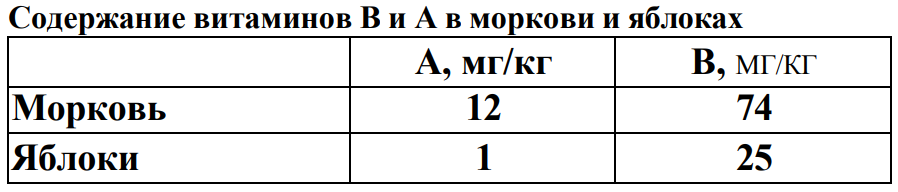
\includegraphics[scale=0.5]{img1.png}
	$$
	\subsection*{Построение математической модели}
	Человеку необходимо спланировать потребление витаминов так, чтобы минимизировать стоимость покупки овощей. Введем переменные для модели:
	\begin{itemize}
		\item $x_1$ --- количество моркови, кг;
		\item $x_2$ --- количество яблок, кг.
	\end{itemize}
	Суммарная стоимость при покупке всех типов овощей составляет $$f(x_1, x_2) = 100x_1 + 200x_2.$$
	Эта функция и будет являться целевой функцией, определяющей суммарную стоимость овощей, которую мы должны минимизировать.\\\\
	Введем ограничения для переменных $x_1$ и $x_2$. Количество килограмм овощей не может быть отрицательным, поэтому $$x_1 \geq 0,\ x_2 \geq 0.$$
	Содержание витаминов в моркови и яблоках ограничено, но не должно быть ниже порогового значения: для витамина А $$12 x_1 + x_2 \geq 10;$$
	для витамина В $$74x_1 + 25 x_2 \geq 90.$$
	Таким образом, итоговая математическая модель имеет вид:
	$$f(x_1, x_2) = 100x_1 + 200x_2 \to \min$$
	$$\begin{cases}
		12 x_1 + x_2 \geq 10,\\
		74x_1 + 25 x_2 \geq 90;
	\end{cases}$$
	$$x_1 \geq 0,\ x_2 \geq 0.$$
	Она описывает задачу линейного программирования.
	\subsection*{Реализация математической модели в форме файла .mod}
	Файл модели model.mod имеет следующую структуру:
	\listinginput[1]{1}{model.mod}
	\subsection*{Решение оптимизационной задачи средствами AMPL}
	Файл запуска lp.run имеет следующую структуру:
	\listinginput[1]{1}{lp.run}
	Ответ в окне консоли:
	\begin{verbatim}
		ampl: include lp.run
		CPLEX 22.1.1.0: optimal solution; objective 121.6216216
		0 dual simplex iterations (0 in phase I)
		cost = 121.622
		
		carrot = 1.21622
		
		apple = 0
	\end{verbatim}
	Таким образом, минимальная стоимость овощей будет равна $121.622$ руб. И для этого нужно купить $1.21622$ кг моркови и $0$ кг яблок.
\end{document}